% !Mode:: "TeX:UTF-8"
% !TEX program  = xelatex
\section{Question 1}
\begin{statebox}{Two important facts}{question-1}
    \begin{align*}
        N'(x) &= \frac{1}{\sqrt{2\pi}}\exp\left(\frac{x^2}{2}\right) \\
        SN'(d_1) &= \exp\left(-r(T-t)\right)EN'(d_2)
    \end{align*}
\end{statebox}

\begin{figure}[H]
    \centering
    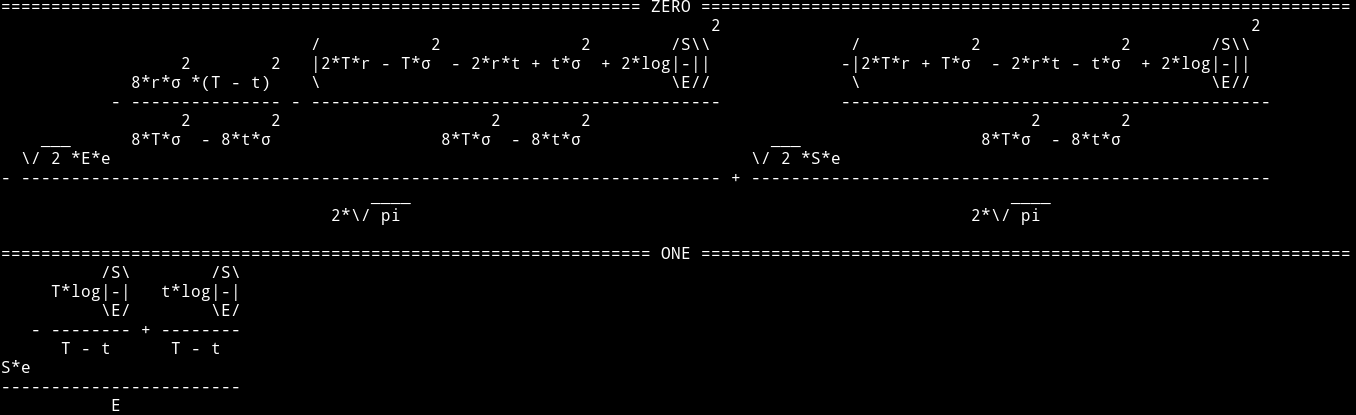
\includegraphics[width=\textwidth]{figures/2019-11-14-derivation-1}
    \caption{公式符号推导结果}\label{F:derivation-1}
\end{figure}

首先, 我们尝试使用符号推导解决问题, 基于 \texttt{sympy} 库的程序请参见附录~\ref{A:1}. 运行结果如图~\ref{F:derivation-1}. 可以看出, 如果不经变换使用符号计算, 是得不到答案的; 经过如式~\eqref{E:1}变换:
\begin{equation}\label{E:1}
    \log\left(\frac{SN'(d_1)}{\exp\left(-r(T-t)\right)EN'(d_2)}\right),
\end{equation}
符号简化到如式~\eqref{E:2}, 此时符号推导已经进行不下去了, 通过人为演算可以发现式~\eqref{E:2}恒等于1, 因此等式成立.
\begin{equation}\label{E:2}
    S\exp\left(-\frac{T\log\left(\frac{S}{E}\right)}{T-t} + \frac{t\log\left(\frac{S}{E}\right)}{T-t}\right),
\end{equation}

最后, 我们采用人工推导, 如式~\eqref{E:3}.
\begin{equation}\label{E:3}
    \begin{aligned}
        \log\left(\frac{SN'(d_1)}{\exp\left(-r(T-t)\right)EN'(d_2)}\right) &= \log\left(\frac{S\frac{1}{\sqrt{2\pi}}\exp\left(-\frac{d_1^2}{2}\right)}{\exp\left(-r(T-t)\right)E\frac{1}{\sqrt{2\pi}}\exp\left(-\frac{d_2^2}{2}\right)}\right) \\
        &= \log\left(\frac{S}{E}\right) + r(T-t) - \frac{1}{2}\left(d_1^2-d_2^2\right) \\
        &= \log\left(\frac{S}{E}\right) + r(T-t) - \frac{1}{2}(d_1+d_2)(d_1-d_2) \\
        &= \log\left(\frac{S}{E}\right) + r(T-t) - \frac{1}{2}\frac{2\log\left(\frac{S}{E}\right)+2r(T-t)}{\sigma\sqrt{T-t}}\frac{\sigma^2(T-t)}{\sigma\sqrt{T-t}} \\
        &= \log\left(\frac{S}{E}\right) + r(T-t) - \frac{1}{2}\left(2\log\left(\frac{S}{E}\right)+2r(T-t)\right) \\
        &= 0
    \end{aligned}
\end{equation}



\section{Question 2}
\begin{statebox}{Symbolic Derivation}{question-2}
    \begin{enumerate}
        \item Adapt function \texttt{lect7\_1.m} to return more Greeks.
        \item Investigate the use of \texttt{MATLAB}'s symbolic toolbox to confirm the results in this lecture.
    \end{enumerate}
\end{statebox}

\noindent\commandbox{greeks('S', 'E', 'r', 'sigma', 'tau', to_simple=True, to_latex=True)}

代码详见附录~\ref{A:2}, 运行结果如式~\ref{E:4}与式~\ref{E:5} (可能不美观).
\begin{equation}\label{E:4}
    \begin{aligned}
        C &= S\,\left(\frac{\mathrm{erf}\left(\frac{\sqrt{2}\,\left(\ln\left(\frac{S}{E}\right)+\tau \,\left(\frac{\sigma ^2}{2}+r\right)\right)}{2\,\sigma \,\sqrt{\tau }}\right)}{2}+\frac{1}{2}\right)+E\,{\mathrm{e}}^{-r\,\tau }\,\left(\frac{\mathrm{erf}\left(\frac{\sqrt{2}\,\left(\sigma \,\sqrt{\tau }-\frac{\ln\left(\frac{S}{E}\right)+\tau \,\left(\frac{\sigma ^2}{2}+r\right)}{\sigma \,\sqrt{\tau }}\right)}{2}\right)}{2}-\frac{1}{2}\right) \\
        C\delta &= \frac{\mathrm{erf}\left(\frac{\sqrt{2}\,\left(\ln\left(\frac{S}{E}\right)+\tau \,\left(\frac{\sigma ^2}{2}+r\right)\right)}{2\,\sigma \,\sqrt{\tau }}\right)}{2}+\frac{1}{2} \\
        C\nu &= \frac{7186705221432913\,S\,\sqrt{\tau }\,{\mathrm{e}}^{-\frac{{\left(\ln\left(\frac{S}{E}\right)+\tau \,\left(\frac{\sigma ^2}{2}+r\right)\right)}^2}{2\,\sigma ^2\,\tau }}}{18014398509481984} \\
        C\theta &= E\,r\,{\mathrm{e}}^{-r\,\tau }\,\left(\frac{\mathrm{erf}\left(\frac{\sqrt{2}\,\left(\sigma \,\sqrt{\tau }-\frac{\ln\left(\frac{S}{E}\right)+\tau \,\left(\frac{\sigma ^2}{2}+r\right)}{\sigma \,\sqrt{\tau }}\right)}{2}\right)}{2}-\frac{1}{2}\right)-\frac{7186705221432913\,S\,\sigma \,{\mathrm{e}}^{-\frac{{\left(\ln\left(\frac{S}{E}\right)+\tau \,\left(\frac{\sigma ^2}{2}+r\right)\right)}^2}{2\,\sigma ^2\,\tau }}}{36028797018963968\,\sqrt{\tau }} \\
        C\rho &= E\,\tau \,{\mathrm{e}}^{-r\,\tau }\,\left(\frac{\mathrm{erf}\left(\frac{\sqrt{2}\,\left(-\tau \,\sigma ^2+2\,\ln\left(\frac{S}{E}\right)+2\,r\,\tau \right)}{4\,\sigma \,\sqrt{\tau }}\right)}{2}+\frac{1}{2}\right) \\
        C\gamma &= \frac{7186705221432913\,{\mathrm{e}}^{-\frac{{\left(\ln\left(\frac{S}{E}\right)+\tau \,\left(\frac{\sigma ^2}{2}+r\right)\right)}^2}{2\,\sigma ^2\,\tau }}}{18014398509481984\,S\,\sigma \,\sqrt{\tau }} \\
    \end{aligned}
\end{equation}

\begin{equation}\label{E:5}
    \begin{aligned}
        P &= \frac{E\,{\mathrm{e}}^{-r\,\tau }}{2}-\frac{S}{2}+\frac{S\,\mathrm{erf}\left(\frac{\sqrt{2}\,\left(\ln\left(\frac{S}{E}\right)+\tau \,\left(\frac{\sigma ^2}{2}+r\right)\right)}{2\,\sigma \,\sqrt{\tau }}\right)}{2}+\frac{E\,\mathrm{erf}\left(\frac{\sqrt{2}\,\left(\sigma \,\sqrt{\tau }-\frac{\ln\left(\frac{S}{E}\right)+\tau \,\left(\frac{\sigma ^2}{2}+r\right)}{\sigma \,\sqrt{\tau }}\right)}{2}\right)\,{\mathrm{e}}^{-r\,\tau }}{2} \\
        P\delta &= \frac{\mathrm{erf}\left(\frac{\sqrt{2}\,\left(\ln\left(\frac{S}{E}\right)+\tau \,\left(\frac{\sigma ^2}{2}+r\right)\right)}{2\,\sigma \,\sqrt{\tau }}\right)}{2}+\frac{1}{2} \\
        P\nu &= \frac{7186705221432913\,S\,\sqrt{\tau }\,{\mathrm{e}}^{-\frac{{\left(\ln\left(\frac{S}{E}\right)+\tau \,\left(\frac{\sigma ^2}{2}+r\right)\right)}^2}{2\,\sigma ^2\,\tau }}}{18014398509481984} \\
        P\theta &= E\,r\,{\mathrm{e}}^{-r\,\tau }\,\left(\frac{\mathrm{erf}\left(\frac{\sqrt{2}\,\left(\sigma \,\sqrt{\tau }-\frac{\ln\left(\frac{S}{E}\right)+\tau \,\left(\frac{\sigma ^2}{2}+r\right)}{\sigma \,\sqrt{\tau }}\right)}{2}\right)}{2}-\frac{1}{2}\right)-\frac{7186705221432913\,S\,\sigma \,{\mathrm{e}}^{-\frac{{\left(\ln\left(\frac{S}{E}\right)+\tau \,\left(\frac{\sigma ^2}{2}+r\right)\right)}^2}{2\,\sigma ^2\,\tau }}}{36028797018963968\,\sqrt{\tau }} \\
        P\rho &= E\,\tau \,{\mathrm{e}}^{-r\,\tau }\,\left(\frac{\mathrm{erf}\left(\frac{\sqrt{2}\,\left(-\tau \,\sigma ^2+2\,\ln\left(\frac{S}{E}\right)+2\,r\,\tau \right)}{4\,\sigma \,\sqrt{\tau }}\right)}{2}+\frac{1}{2}\right) \\
        P\gamma &= \frac{7186705221432913\,{\mathrm{e}}^{-\frac{{\left(\ln\left(\frac{S}{E}\right)+\tau \,\left(\frac{\sigma ^2}{2}+r\right)\right)}^2}{2\,\sigma ^2\,\tau }}}{18014398509481984\,S\,\sigma \,\sqrt{\tau }}
    \end{aligned}
\end{equation}



\clearpage
\appendix
    \section{附录: 问题一 \texttt{Python} 代码}\label{A:1}
        \Python{8-a.py}{code/8-a.py}
    \section{附录: 问题二 \texttt{Python} 代码}\label{A:2}
        \Python{8-b.py}{code/8-b.py}
        \Python{8-b.py}{code/8-b_MATLAB.py}
